\documentclass[sigconf,review,anonymous]{acmart}
\setcopyright{rightsretained}

\usepackage{listings}
\usepackage{dirtree}
\usepackage{hyperref}
\usepackage{booktabs}
\usepackage{url}
\usepackage[utf8]{inputenc}
\usepackage{tikz}
\usepackage{graphicx}
\usepackage{mathtools}
\usepackage{float}
\usepackage{amsthm}
\usepackage{amsmath}
\usepackage{amsfonts}
\usepackage{bbm}
\usepackage[scientific-notation=true]{siunitx}

\usepackage{amssymb}
\usepackage{tabulary}

\usepackage{etoolbox}

\usepackage{algorithm}
\usepackage{algorithmic}

\makeatletter
\newcommand\fs@norules{\def\@fs@cfont{\bfseries}\let\@fs@capt\floatc@ruled
  \def\@fs@pre{}%
  \def\@fs@post{}%
  \def\@fs@mid{\kern3pt}%
  \let\@fs@iftopcapt\iftrue}
\makeatother
\floatstyle{norules}
\restylefloat{algorithm}

\let\tinymatrix\smallmatrix
\let\endtinymatrix\endsmallmatrix
\patchcmd{\tinymatrix}{\scriptstyle}{\scriptscriptstyle}{}{}
\patchcmd{\tinymatrix}{\scriptstyle}{\scriptscriptstyle}{}{}
\patchcmd{\tinymatrix}{\vcenter}{\vtop}{}{}
\patchcmd{\tinymatrix}{\bgroup}{\bgroup\scriptsize}{}{}

\newcommand{\ra}[1]{\renewcommand{\arraystretch}{#1}}

\usepackage[draft,index]{fixme}
\fxsetup{theme=color,mode=multiuser,layout=inline,draft}

% correct bad hyphenation here
%\hyphenation{op-tical net-works semi-conduc-tor}

\begin{document}
%
% paper title
% can use linebreaks \\ within to get better formatting as desired
\title{Online (Bandit) Policy Selection for EASY-Backfilling}

\author{Eric Gaussier}
\affiliation{%
  \institution{Univ. Grenoble Alpes, CNRS, Grenoble INP, LIG}
  \country{France}}
\email{eric.gaussier@imag.fr}
\author{J\'er\^ome Lelong}
\affiliation{%
  \institution{Univ. Grenoble Alpes, Inria, CNRS, Grenoble INP, LJK}
  \country{France}}
\email{jerome.lelong@imag.fr}
\author{Valentin Reis}
\affiliation{%
  \institution{Univ. Grenoble Alpes, Inria, CNRS, Grenoble INP, LIG}
  \country{France}}
\email{valentin.reis@imag.fr}
\author{Denis Trystram}
\affiliation{%
  \institution{Univ. Grenoble Alpes, Inria, CNRS, Grenoble INP, LIG}
  \country{France}}
\email{denis.trystram@imag.fr}

\begin{abstract}

  The EASY-FCFS heuristic is the basic building block of job scheduling
  policies in most parallel High Performance Computing (HPC) platforms. Despite
  its good properties (simplicity, no starvation), it could still be improved
  on a per-system basis. This tuning process is difficult because of
  non-linearities in the scheduling process. The study proposed here considers
  an online approach to the automatic tuning of the EASY heuristic for HPC
  platforms. More precisely, we consider the problem of selecting a reordering
  policy of the job queue under several feedback modes. We show via a
  comprehensive experimental campaign that noisy feedback (using a weak
  simulator) recovers existing in-hindsight results that allow to divide the
  average waiting time up to a factor of 2. Moreover, we show that bandit
  feedback can be used by a simple multi-armed bandit algorithm to decrease the
  average waiting time down to 40\% of its original value without using a
  simulator.

\end{abstract}

\maketitle


\section{Introduction}
\label{sec:intro}

\subsection{Context}

Providing the computing infrastuctures needed to solve actual complex problems
arising in the various fields of modern society (including climate change,
health, green energy or security) is a strategic challenge. The main pillar of
the answer to this challenge is to build extreme-scale parallel and distributed
platforms. The never-ending race for more computing power and storage capacity does
not only lead to sophisticated specific Exascale platforms, but the objective
of the community is to design efficient sustained Petascale platforms. This
large-scale evolution and the increasing complexity in both architecture and
applications create many scientific and technical problems. Accordingly, system
management software still has a long way to go. The existing job and resource
management softwares allow to run tens of thousands of jobs on hundreds of thousands
of cores. They are based on robust policies, however, despite their positive
properties such as relative simplicity and prevention of job starvation,
there is still room for improvement. We propose here to study how to tune the
ordering of the submission queues in the frame of the classical
EASY-BackFilling family of heuristics using two new online learning approaches
(an approach based on a simulator and an approach using multi-armed bandit).

Most common work in the literature consider \textit{a posteriori} optimization
of a scheduling algorithm on a (actual) data set.  The increasing amount and
diversity of data generated by large scale platforms motivate the community to
study more sophisticated policies that could leverage these data.  During the
last few years, there was an explosion of the number of works at the interface
of HPC and BigData fields, dealing with learning algorithms. Recent
sophisticated approaches developed \textit{ad hoc} supervised machine learning
algorithms for reducing uncertainty in problem parameters (e.g. job execution
times, memory requirements, etc.) via prediction. However, only few studies
evaluate the impact of such techniques on the performances of the resource
manager.

Contrarily to most existing studies, which consider the learning of specific
parameters of a trace, we provide a complete system that uses feedback from the
system for adapting the whole behavior online.  Our focus within this work is
to learn how the management system behaves within the usual framework of
EASY-BF. More precisely, we provide strategies for choosing the most
appropriate queue reordering policy to be used for job selection. This approach
is assessed by an extensive resampling-based experimental campaign that uses 7
actual traces.

\subsection{Contributions}

Our main contribution is to investigate two original methods for learning a
good scheduling policy on a per-system basis. We focus in this work on the
average waiting time of the jobs. Each method aims to choose the best queue
reordering policy in a fixed search set of semantically diverse options.

The first method (full feedback) continuously uses simulation on data gathered
from the past and current system workload. In order to reflect the
uncertainties in the data, we also evaluate a more realistic "noisy" variant in
which simulations are imprecise.

The second method (bandit feedback) is a simulator-less approach based on a
multi-armed bandit algorithm that derives feedback by measuring system
performance.

Both of these methods are evaluated with a specially developped simulator that is
open-sourced and packaged for the community.


Our main results are as follows: The approach based on the simulator provides
very good results, close to the best policy in the search set. In essence, this
means that we are able to recover in an online fashion existing results that
divide average waiting times by factor of \textcolor{orange}{X} to
\textcolor{orange}{X}. Indeed, we show that the required sample sizes for
policy selection in batch schedulers are small enough for workload resampling to
be avoided in practice. The variant based on noisy data, which is closer to
actual conditions of uncertainties on both jobs and platform, also behaves very
well. The alternate approach based on a multi-armed bandit also provides
reasonable results at a much lower cost, dividing the average waiting times by
a factor of \textcolor{orange}{X} to \textcolor{orange}{X}.

Let us emphasize the main results of this study: While the First-Come,
First-Serve approach to minimizing the waiting times is a common default
strategy, it can absolutely be outperformed.  We show how to automate selection
of a good alternative policy in two cases (depending whether a simulator is
available or not), and provide the difference in performance to be expected
between both situations.

\section{Related Work}
\label{sec:rw}

This section presents and discuss the most significant results related to job
scheduling and learning algorithms in this context.  Let us start by recalling
some basics about scheduling heuristics in HPC platforms:

Parallel job scheduling is a old studied theoretical
problem~\cite{Frachtenberg:2009:JSS:1692356,Feitelson:2004:PJS:2128864.2128865}
whose practical ramifications, varying hypotheses, and inherent uncertainty of
the problem applied on the HPC field have driven practitioners to use simple
heuristics (and researchers to study their behavior). The two most popular
heuristics for HPC platforms are EASY~\cite{easy} and
Conservative~\cite{Mu'alem:2001:UPW:380314.380315} backfillings.

While Conservative Backfilling offers many advantages~\cite{bfchar}, it has a
significant computational overhead, which mainly explains why most of the
machines of the top500 ranking~\cite{top500} rather use a variant of EASY-BF
instead.  There is a large body of work seeking to improve/tune EASY. Indeed,
while the basic mechanism is used by some actual resource and job management
softwares (most notably SLURM~\cite{SLURMdocSCHED}), this is rarely done
without fine tunings by system administrators.

The original EASY mechanism refers to a First-Come-First-Serve basis.  Several
works explore how to tune EASY by reordering waiting and/or backfilling
queues~\cite{Tsafrir_easypp_2005}, sometimes even in a randomized
manner~\cite{1592720}, as well as some implementations~\cite{Jackson2001}.
However, as successful as they may be, these works do not address the
dependency of scheduling metrics on the workload~\cite{variability}. Indeed
these studies most often report \textit{post-hoc} performance since they
compare algorithms after the workload is known.

The dynP scheduler~\cite{streit_selftuning_2002} proposes a systematic
method to tuning these queues, although it requires simulated scheduling runs
at decision time and therefore, it costs much more than the natural execution of EASY.

\subsection{Data-aware resource management.}

There was a recent focus on leveraging the huge amount of data available in
large scale computing platforms in order to improve system performance. Some
works use collaborative filtering to colocate tasks in clouds by estimating
application interference~\cite{7516031}. Some others are closer to the
application level. For instance, ~\cite{fmodeling} uses binary classification
to distinguish benign memory faults from application errors in order to execute
recovery algorithms.

Several works use similar techniques in the context of HPC, in
particular~\cite{Tsafrir_easypp_2005,learningruntimes}, hoping that better job
runtime estimations should improve the scheduling~\cite{chiang_impact_2002}.
Some algorithms estimate runtime distributions model and choose jobs using
probabilistic integration procedures~\cite{Nissimov2008}.  However, these works
do not address the duality between the cumulative and maximal scheduling costs,
as mentioned in~\cite{learningruntimes}. While these previous works intend to
estimate uncertain parameters, we consider here a more pragmatic approach,
which directly learn a good scheduling policy from a given policy space.

Existing work~\cite{jsspp17} takes this approach in an offline manner, by
splitting workload data in a training/testing fashion. This work studied
EASY-Backfilling and shows that the relative performance of some well-known
priority orders for starting jobs differs between workloads, but is relatively
stable troughout time for a given workload.

\subsection{Multi-Armed Bandits.}

A multi-armed bandit (MAB) problem is a sequential allocation problem with
partially observable rewards. At every round, an action (represented by an arm
of the Bandit) must be chosen in a fixed set and the corresponding reward is
observed. The goal of a MAB algorithm is to maximize the total reward obtained
in a successive number of rounds.  There exist a bunch of works that address
this problem under a variety of constraints, The two most popular settings are
the original stochastic  case and the adversarial case. See~\cite{thompson} for
the original work on the stochastic case and~\cite{Auer2002} for the "Upper
Confidence Bound" family of algorithms. According to our knowledge, the work
of~\cite{Banos} is the earliest known work to us for the adversarial case
see~\cite{nonstoch} for the "Exponential-weight" family of algorithms. We refer
to the review~\cite{bubnow} for a comprehensive overview of the field. While
these algorithms bound the cumulative difference in loss to the best arm (the
regret), they have functional constraints such as the fact that the rewards
should be contained in a range. A simple heuristic called
\textit{Epsilon-Greedy} introduced in~\cite{Auer2002} is known to achieve good
results in practice, and does not have this requirement.

%%%%%%%%%%%%%%%%%%%%%%%%%%%%%%%%%%%%%%%%%%%%%%%%%%

\section{Problem setting}
\label{sec:problem_setting}

%This section presents the systems under study and the scheduling problem.  It
%first introduces the EASY-Backfilling heuristic and gives \todo{fix} the
%problem statement.

\subsection{System Description}
\label{sub:sysdesc}

The crucial part of batch scheduling software is the scheduling algorithm that
determines where and when the submitted jobs are executed. The process is as
follows: jobs are submitted by end-users and queued until the scheduler selects
one of them for running. Each job has a provided bound on the execution time
and some resource requirements (number and type of processing units). Then, the
RJMS drives the search for the resources required to execute this job. Finally,
the tasks of the job are assigned to the chosen nodes.

In the classical case, the management software needs to execute a set of
concurrent parallel jobs with rigid (known and fixed) resource requirements on
a HPC platform represented by a pool of $m$ identical resources. This is an
on-line problem since the jobs are submitted over time and their
characteristics are only known when they are released.  Below is the brief
description (with the corresponding notations) of the characteristics of job
$j$:

\begin{itemize}

   \item Submission date $r_j$ (also called \textit{release date})

   \item Resource requirement $q_j$ (number of processors)

   \item Actual running time $p_j$ (sometimes called \textit{processing time})

   \item Requested running time $\widetilde{p_j}$ (sometimes called
     \textit{walltime}), which is an upper bound of $p_j$.

\end{itemize}

The resource requirement $q_j$ of job $j$ is known when the job is submitted at
time $r_j$, while the requested running time $\widetilde{p_j}$ is given by the
user as an estimate. Its actual value $p_j$ is only known \textit{a posteriori}
when the job really completes.  Moreover, the users have incentive to
over-estimate the actual values, since jobs may be ``killed'' if they surpass
the provided value.

\subsection{Brief description of EASY Backfilling}
\label{sub:easy}

The selection of the job to run is performed according to a scheduling policy
that establishes the order in which the jobs are executed.  EASY-Backfilling is
the most widely used policy due to its simple and robust implementation and
known benefits such as high system utilization~\cite{easy}. This strategy has
no worst case guarantee beyond the absence of starvation (i.e. every job will
be scheduled at some moment).

The EASY-FCFS heuristic uses a job queue to select and backfill jobs.  At any
time that requires a scheduling decision (i.e. job submission or termination),
the scheduler goes through the job queue in First-Come,First-Serve (FCFS) order
and starts jobs until it finds a job that can not be started right away. It
then makes a reservation for this job at the earliest predictable time and
starts \textit{backfilling} the job queue in FCFS order, starting any job that
does not delay the unique reservation.

\subsection{Scheduling Objective}
\label{sub:scheduling_objectives}

A system administrator may use one or multiple cost metric(s). Our study of
scheduling performance relies on the waiting times of the jobs, which is one of
the more commonly used objectives.

     \begin{equation}
       \textbf{Wait}_j =  start_j-r_j
     \end{equation}

Like other cost metrics, the waiting time is usually considered in its
\textit{cumulative} version, which means that one seeks to minimize the average
waiting time (\textbf{AvgWait}). It is worth noting that the \textbf{MaxWait},
a.k.a the maximal value of the waiting time of all the jobs is also worthy of
interest. Unfortunately, these criteria are antagonistic in nature. Section~\ref{sub:th} will outline our
approach to address the bi-objective aspect of this problem.




\section{Tuning EASY by reordering and thresholding the job queue}
\label{sec:framework}

This section presents two mechanisms for safely tuning the EASY-Backfilling:
job queue reordering and job thresholding. Together, these two building blocks
constitute a robust framework for tuning EASY.

\subsection{Reordering the job Queue}
\label{subsec:policies}

The EASY heuristic uses a job queue to select and backfill jobs. While this job
queue is ordered in FCFS order in the original heuristic, it is possible to
reorder it at will. We settle on a reasonable search space of 10 reordering policies.

\begin{enumerate}
  \item FCFS: First-Come First-Serve, which is the widely used default policy~\cite{easy}.
  \item LCFS: Last-Come First-Serve.
  \item SPF: Smallest estimated Processing time $\widetilde{p_{j}}$ First ~\cite{bfchar}.
  \item LPF: Longest estimated Processing time First.
  \item LQF: Largest resource requirement $q_j$ First.
  \item SQF: Smallest resource requirement First.
  \item LEXP: Largest Expansion Factor First~\cite{bfchar}, where the expansion
    factor is defined as follows:
  \begin{equation} \frac{start_j - r_j + \widetilde{p_j}}{\widetilde{p_j}} \end{equation}
  where $start_j$ is the starting time of job $j$.
  \item SEXP: Smallest Expansion Factor First
  \item LRF: Largest Ratio $\frac{p_j}{q_j}$ First
  \item SRF: Smallest Ratio First
  \item LAF: Largest Area $ p_j \times q_j$ First
  \item SAF: Smallest Area First
\end{enumerate}

This search space is designed with the goal of being as semantically diverse as
possible without making any judgement on which policy should perform well in
practice. In the following, we denote these policies by $P_i$ with $i = 1
\ldots 12$.

\subsection{Thresholding}
\label{sub:th}
As existing works point out, reordering the job queue means losing the
no-starvation guarantee and some individual jobs therefore can wait an undue
amount of time. It is possible to introduce a thresholding mechanism in order
to prevent this behavior: When a job's \textit{waiting time so far} exceeds a
fixed threshold $\Theta$, it is jumped at the head of the queue. We denote by
EASY($P,\Theta$) the scheduling policy that starts and backfill jobs according to
the (thresholded) reordering policy $P$. For the sake of completeness,
Algorithm~\ref{alg:EASY} describes the EASY($P,\Theta$) heuristic.

\begin{algorithm}[]
  \caption{EASY($P,\Theta$) policy}
  \begin{algorithmic}[1]
    \renewcommand{\algorithmicrequire}{\textbf{Input:}}
    \renewcommand{\algorithmicensure}{\textbf{Output:}}
    \REQUIRE Queue $Q$ of waiting jobs.
    \ENSURE None (calls to $Start()$)
    \STATE Sort $Q$ according to $P_R$
    \STATE Move all jobs of $Q$ for which $wait_j > \Theta$ ahead
    of the queue (breaking ties in FCFS order).
    \\ \textit{Starting jobs until the machine is full}
    \FOR {job $j$ in Q do}
    \IF {$j$ can be started given the current system use.}
    \STATE Pop $j$ from Q
    \STATE $Start(j)$
    \ELSE
    \STATE Reserve $j$ at the earliest
    time possible according to the estimated running times
    of the currently running jobs.
    \\ \textit{Backfilling jobs}
    \FOR {job $j'$ in $Q\setminus\{j\}$}
    \IF {$j'$ can be started without delaying the reservation on $j$.}
    \STATE Pop $j'$ from $Q$
    \STATE $Start(j')$
    \ENDIF
    \ENDFOR
    \STATE \textbf{break}
    \ENDIF
    \ENDFOR
  \end{algorithmic}
  \label{alg:EASY}
\end{algorithm}


\section{Online tuning}
\label{sec:online}

\begin{figure*}[]
  \centering
  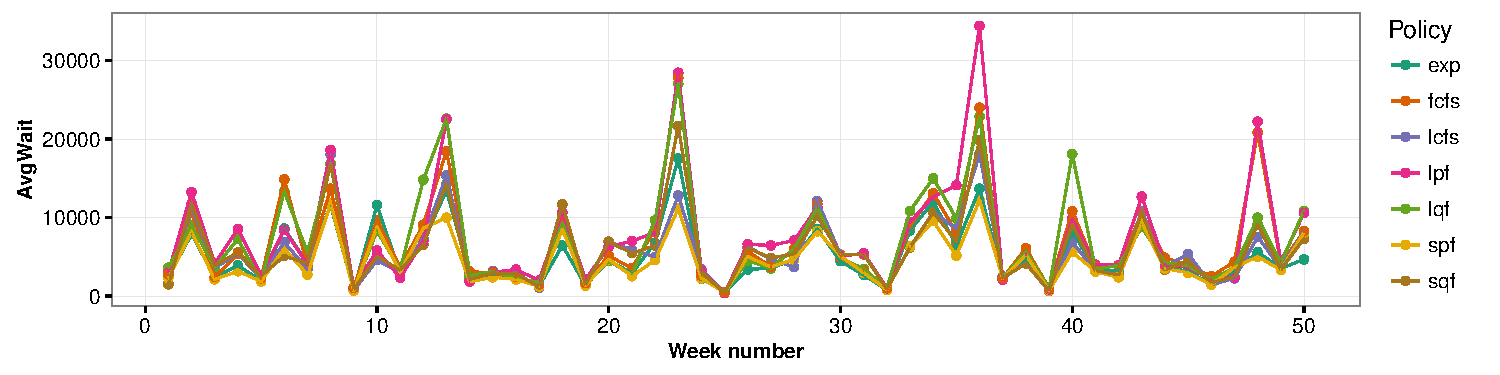
\includegraphics[scale=0.6]{figures/variability.pdf}

  \caption{Variability in the weekly average waiting time in the KTH-SP2 trace
  (see Subsection~\ref{sub:traces}) for 7 different policies. The policy set is
  reduced as not to obstruct the figure.}

  \label{fig:variability}
\end{figure*}

We present here the strategies we have retained for selecting a policy. We will
refer to the period during which a selected policy is applied as the
\textit{policy period} and will denote the length of this period as $\Delta$.
The time interval is thus divided into periods of equal lengths ($\Delta$):
$\Delta_0, \cdots, \Delta_T$, where $T$ is the index of the current policy
period. A new policy is selected at the beginning of each period and applied
during the whole period.

We further assume that there is a certain regularity among periods,
\textit{i.e.} that the distributions underlying the jobs submitted do not
radically differ between consecutive periods. This assumption is validated in
the study presented in~\cite{jsspp17}. It further entails that the behavior of
a policy on the previous periods reflects its behavior on the current one, so
that the selection of a policy can be based on its behavior on previous
periods. However, there may be some variability between different periods for
certain cost metrics~\cite{feitelson2001metrics}. This is illustrated in
Figure~\ref{fig:mosn} which displays the average waiting time of various
policies for the KTH-SP2 trace (see~\ref{sub:traces} for a description of the
workloads) using weekly periods encompassing one year. As one can note, the
average waiting time varies a lot from one week to the other, for all the 7
policies considered. This indicates that when when the cost metric is averaged
over different periods, there is a tradeoff to find in between longer periods
that would somehow limit the variability, and shorter ones that yield more
values for the estimation. We will come back to this issue below.

The selection of a policy is of course reminiscent of reinforcement learning.
It is important to note, however, that a pure reinforcement learning approach
is difficult to develop in our context. Indeed, while we have outlined a
reduced action space, the state space to consider is infinite. This is not
prohibitive \textit{per se}, as modern methods~\cite{aprl}
can bypass dimensionality issues via function approximation. However, these
methods rely on large amounts of data, and we are studying online (often called
\textit{on-policy} methods in reinforcement learning) methods. We rely here on
simpler, yet we believe more effective, strategies to solve this problem.
These strategies are applied online and rely on exact simulation, noisy
simulation and $\epsilon$-greedy bandit exploration.

\subsection{Policy selection with exact simulation}
\label{sub:feedback}

Several simulators have been developed for "playing" reordering policies on a
given set of jobs. We rely in this study on a lightweight simulator (see
Section~\ref{sec:experiments}) that can efficiently simulate different
policies. Such simulators are interesting inasmuch as they provide an estimate
of the cost of a given policy on a set of jobs, as described below.

Let $l(\Delta_t)$ denote the number of jobs \textit{submitted} during the
period $\Delta_t$ ($0 \le t < T$), and $P_i$ ($1 \le i \le 12$) one reordering
policy (defined in Section~\ref{subsec:policies}). The cost of policy $P_i$
during the period $\Delta_t$ is defined as:
%
\begin{equation} \label{eq:cost-exact} w_{\mbox{exact}}(t;P_i) =
\sum_{j=1}^{l(\Delta_t)} \mbox{Wait}_j^{P_i} \end{equation}
%
where $\mbox{Wait}_j^{P_i}$ denotes the estimate provided by the simulator of
the waiting time for job $j$ according to policy $P_i$. The estimation of the
cost of a policy over all the periods preceding the current period can then be
defined as:
%
\begin{equation} \label{eq:tot-cost-exact} w(\rightarrow T;P_i) =
\sum_{t=0}^{T-1} \lambda^{T-1-t} w_{\mbox{exact}}(t;P_i) \end{equation}
%
$\lambda \in [0,1]$ is a decay parameter that can be used to privilege recent
history (\textit{i.e.} recent periods). One then selects the policy $P$ that
minimizes the above cost for the period $\Delta_T$:
%
\begin{equation} \label{eq:select-exact} P = \mbox{argmin}_{P_i, 1 \le i \le
12} w(\rightarrow T;P_i) \end{equation}

The above cost directly corresponds to the cumulative waiting time of the
policy over the preceding periods (more precisely to the cumulative simulated
estimate of the waiting time of the policy over the preceding periods) so that
the length of the period has little impact here. The only bias comes from the
boundary states of the simulation. Indeed, we run simulations from an empty
system and wait for the system to be empty when job submissions cease at the
end of the submission period.

Furthermore, in the context of this study and as detailed in
Section~\ref{sec:experiments}, we rely on averages over several execution
traces in order to obtain reliable estimate of the behavior of different
policies and policy selection strategies. Such traces are typically obtained by
simulation. Using the same simulator for generating the traces and estimating
the cost as defined in Eqs \ref{eq:cost-exact} and \ref{eq:tot-cost-exact}
would however be too optimistic and would represent an upper bound on what can
be achieved by a selection strategy based on simulation. In order to have a
more realistic estimate of the behavior of a selection strategy based on
simulation, we introduce noise in the simulator, as described below.

\subsection{Policy selection with noisy simulation}
\label{sub:noisy}

In order to simulate how the simulation strategy for selecting policies would
work on non simulated traces, we randomly introduce noise in the estimate of
the waiting time defined by Eq.~\ref{eq:cost-exact} by rescaling it, either
down or up, for each job:
%
\begin{equation} \label{eq:cost-noisy} w_{\mbox{noisy}}(t;P_i) =
\sum_{j=1}^{l(\Delta_t)} \rho_j \, \mbox{Wait}_j^{P_i} \end{equation}
%
where $\rho$ is uniformly sampled in the interval $[0.85,1.15]$, thus adding a
+/-15\% noise on the waiting time estimated by the simulator. The overall cost
is then defined in the same way as before, leading to:
%
\begin{equation} \label{eq:tot-cost-noisy} w(\rightarrow T;P_i) =
\sum_{t=0}^{T-1} \lambda^{T-1-t} w_{\mbox{noisy}}(t;P_i) \end{equation}
%
As before (see Eq.~\ref{eq:select-exact}), the policy that minimizes the above
cost is selected for the period $\Delta_T$.

Instead of introducing noise in the output of the simulator when selecting the
policy, one could have introduced it when collecting the execution traces. Our choice
to add the noise after the simulation step is motivated by simplicity. As we
will see in Section~\ref{sec:experiments}, there is little difference between
the two selection methods, which is an important result of our study.

Lastly, as before, the length of the period has little impact here as the cost
metric corresponds to the cumulative simulated waiting time for each policy.

\subsection{Policy selection with $\epsilon$-greedy exploration}
\label{sub:bandit}

The previous strategies estimate the cost of all policies over all previous
periods; the best policy according to this cost is then selected for the
current period, the costs of all policies being updated for the next period.
This is interesting as one maintains a complete knowledge of all policies over
time. However, this requires computing many estimates at each period (as many
as there are policies), which can be time consuming or cumbersome even with
lightweight simulators.

We thus explore here a more efficient strategy that dispenses with estimating
the cost of all policies at a given time and only updates the cost of the
policy that is currently being used. This strategy makes use of the
$\epsilon$-greedy exploration method, standard in reinforcement learning
\cite{Watkins:1989} and bandit problems~\cite{Auer2002}, to tradeoff
exploitation and exploration, and relies, as before, on past estimates of the
cost to select the best policy in the exploitation mode.

Let $l(\Delta_t)$ denote this time the number of jobs \textit{finished} during
the period $\Delta_t$. We define the cost of policy $P_i$ during the period
$\Delta_t$ as:
%
\[ w_{\epsilon}(t;P_i) = \left\{ \begin{array}{ll} \sum_{j=1}^{l(\Delta_t)}
  \textbf{Wait}_j^{P_i} & \mbox{if} \, P_i \, \mbox{used during} \, \Delta_t
  \nonumber\\ 0 & \mbox{otherwise} \end{array} \right.  \]
%
As one can note, the actual waiting time is used here, so that one dispenses
with the use of a simulator for efficiency considerations. This leads to a
faster and easier estimate of the cumulative waiting time, however only for the
policy that is used during $\Delta_t$. Note that there is as previously a bias
due to boundary effects in the measurement method, as we do include jobs that
had been started before $\Delta_t$, as well as disregard jobs that were
submitted during $\Delta_t$ but finish later.

%This also explains the difference
%between the definitions of $l(\Delta_t)$: in the previous selection strategies,
%one relies on a simulated estimate so that jobs need not be finished during
%$\Delta_t$, but only submitted; in contrast, to know their actual waiting time,
%jobs need be finished during $\Delta_t$.

The cost over all previous period of a policy $P_i$ is then defined as:
%
\begin{equation} \label{eq:tot-cost-greedy} w(\rightarrow T;P_i) =
\frac{1}{\sum_{t=0}^{T-1} \mathbbm{1}(P_i,t) l(\Delta_t)} \sum_{t=0}^{T-1}
\mathbbm{1}(P_i,t) \lambda^{T-1-t} w_{\epsilon}(t;P_i) \end{equation}
%
where $\mathbbm{1}(P_i,t) = 1$ if $P_i$ is the policy used during the period
$\Delta_t$ and $0$ otherwise. The normalization by $\sum_{t=0}^{T-1}
\mathbbm{1}(P_i,t) l(\Delta_t)$ is necessary here to ensure that policies
remain comparable over time, as not normalizing would favor the policy that was
first selected, even if this choice was random. This normalization however
entails that the size of the policy period is important: it should not be too
large so as to avoid relying on too few points for estimating the cost, and it
should not be too small to avoid extreme variations between periods. As
explained in Section~\ref{sec:experiments}, we rely in this study on periods of
one day and one week.

The selection of the policy to be used during the current time period
$\Delta_T$ is then based on the standard $\epsilon$-greedy exploration
strategy:

%
\begin{itemize}
\item With probability $(1-\epsilon)$, select the policy $P$ that minimizes the cost over previous time periods (exploitation mode):
%
\begin{equation}
\label{eq:select-greedy}
P = \mbox{argmin}_{P_i, 1 \le i \le 12} w(\rightarrow T;P_i)
\end{equation}
%
\item With probability $\epsilon$, select a policy $P_i, \, 1 \le i \le 12$, at random (exploration mode).
\end{itemize}

Several studies propose to decay $\epsilon$ over time, the exploration being
less important once the estimates for the different policies are reliable
\cite{Tokic:2010}. This strategy has however not been beneficial in our case.
We believe this is due to the properties of the traces we use, as
explained in Section~\ref{sec:experiments}.

\section{Experiments}
\label{sec:experiments}

This section compares the different approaches to policy selection via a
comprehensive experimental campaign.  Subsection~\ref{sub:protocol} outlines
the experimental protocol used and Subsection~\ref{sub:results} contains the
experimental results and their discussion.

\subsection{Experimental Protocol}
\label{sub:protocol}

The Evaluation of computer systems performance is a complex
task. Here, the two main difficulties are choosing a simulation
model and taking into account the variability in the average waiting times.
This section presents our approach, which is based on lightweight simulation
and trace resampling.

\subsubsection{Traces}
\label{sub:traces}

\begin{table}[]
  \centering
  \ra{1.3}
  \caption{Workload logs used in the simulations.}
  \label{tab:logs}
  \begin{tabular}{@{}lrrrr@{}}
    \hline
    Name          & Year & \# MaxProcs & \# Jobs & Duration\\
    \hline
    KTH-SP2       & 1996 & 100         & 28k     & 11 Months\\
    CTC-SP2       & 1996 & 338         & 77k     & 11 Months\\
    SDSC-SP2      & 2000 & 128         & 59k     & 24 Months\\
    SDSC-BLUE     & 2003 & 1,152       & 243k    & 32 Months\\
    ANL-Intrepid  & 2009 & 163840      & 68k     & 9  Months\\
    CEA-Curie     & 2012 & 80,640      & 312k    & 3  Months\\
    Unilu-Gaia    & 2014 & 2,004       & 51k     & 4  Months\\
    \hline
  \end{tabular}
\end{table}

The experimental campaign used in this work uses a mixture of small and large
systems from different periods. Table~\ref{tab:logs} presents the 7 logs, which
can all be obtained from the Parallel Workload
Archive~\cite{Feitelson20142967}. We use the
'cleaned'\footnote{\lstinline[basicstyle=\ttfamily\color{blue}]|http://www.cs.huji.ac.il/labs/parallel/workload/logs.html#clean|}
version of the logs as per the archive. We impose an additional filtering step
to the workloads\footnote{This filtering step is available in the reproducible
workflow\cite{repro} as shell script
\lstinline[basicstyle=\ttfamily\color{blue}]|misc/strong\_filter|} in order to
clean singular data. More precisely, we apply the following modifications:

\begin{enumerate}

  \item If the number of allocated or requested cores of a job  exceeds the
    size of the machine, we remove the job.

  \item If the number of allocated or requested cores is negative, we use the
    available positive value as the request. If both are negative, we remove
    the job.

  \item If the runtime or submission time is negative, we remove the job.

\end{enumerate}

\subsubsection{Simulator}

The choice of a simulator is a critical part of experimental validation that
raises a tradeoff between precision and runtime. High precision can be obtained
by carefully modeling the platform and its network topology, or extracting
information from the jobs from their sources or post-morted logs. This is the
approach used by high-fidelity batch scheduling simulators such as
Batsim~\cite{batsim}. In the present work, the focus is on studying the
EASY-Backfilling mechanism in itself, without adressing the allocation problem.
Moreover, the experimental protocol used here requires many simulation runs.
Therefore, we set the precision/runtime tradeoff at the point which minimizes
simulation runtimes. We discard all topological information relative to the
platform and use the job processing times of the original workloads. In this
setup, the processors are considered to be undistinguishable from each other,
and jobs can be discontinuously mapped to any available processor on the
system. We develop a lightweight simulator\cite{ocst} and an accompanying
multi-armed bandit library\cite{obandit}. See the reproducibility paragraph
below for more information.  With this simulator, we are able to replay
EASY-FCFS on the CEA-CURIE trace in 33 seconds with a machine equipped with an
Intel(R) Core(TM) i5-4310U CPU @ 2.00GHz. As a point of comparison, the Batsim
simulator with no network communication modeling and no resource contiguity
takes more than 7 hours to replay the same trace on the same hardware. The
complete simulation campaign presented below is executed on a single Dell
PowerEdge R730 in 22 hours, including input preparation and analysis code.

\subsubsection{Resampling}
\label{ssub:resampling}

Comparing algorithms in batch scheduling is made especially difficult by the
fluctuations in commonly used metrics~\cite{jsm}. The variability in
performance is known to outrank the available sample sizes: \textit{It is not
enough to simply replay an algorithm using a workload trace}. Indeed, as
presented in Figure~\ref{fig:variability}, the objective function we are using
in this work is subject to high variability. This variability can be so extreme
that even a timeframe of a fews years can be insufficient to compare scheduling
algorithms. In our experience inverting some months in the trace at random can
lead to reversal in the results. This motivated decades of research in workload
modeling~\cite{feitbook}. A recent approach~\cite{feitresampling} proposes to
resample data directly from the original traces. In this work, we use a simple
implementation of these ideas.  More precisely, we want to sample the job
submission process, which is achieved in the following manner: For evey week in
a resampled trace, we iterate over every existing user in the original trace.
For each of these users, we choose a week of the original trace uniformly at
random. The jobs from this user in this original week are chosen to be present
in the week being resampled.  This simple mechanism enables us to preserve the
dependency within a week.  Although the system state may not be independent
from one week to an other, we rely on existing work~\ref{jsspp17} and assume
for these experiments that the system is in a stationary state. While we
do provide guidelines as how to incorporate tracking variant of our algorithms
in~\ref{sec:online} by introducing a decaying discount factor $\lambda$,
this will not be studied in the experiments from this paper, and is left for
future research.

%Thus,
%computing an average over the sampled traces at a given time can be related to
%a time average of an underlying Markov process, which converges to the true
%quantity thanks to the ergodic theorem.  Moreover, the job submission process
%has no long range correlation making it look like an independent and
%identically distributed process when considering sufficiently time spaced
%weeks.

\subsubsection{Experimental campaign}

We use devise the following experimental campaign. For each of the 7 workloads
considered, we use the original data to resample 100 traces, each of a length
of two years. For each resampled trace, we run simulations using the
EASY($P,\Theta$) scheduling heuristic. We fix the value of the job waiting time
threshold $\Theta$ at 40 hours, a sane default. The choice of this default
stems from the analysis developped in ~\cite{jsspp17}. This value is high
enough for queue reorderings to be leveraged while being low enough to provide
the functional requirement of preventing starvation. We simulate
EASY($P,\Theta=40h$) using the following strategies:

\begin{itemize}

  \item All fixed $P_i$ for $1<i<12$ from the search set defined in
    ~\ref{subsec:policies}.  This is done for two reasons. First, it allows to
    see which policy works well for which platform. Second, it allows to
    compare how well strategies proposed in this work with the best
    \textit{a-posteriori} known policy.

  \item The simulation-based ("full feedback") strategy with hyperparameter
    $\Delta \in \left\{ 1 \text{day},1 \text{week} \right\}$. This choice of
    hyperparameter is a consequence of the natural rythm of human activity:
    daily or weekly simulation periods seems to facilitate comparability of
    performance between two periods. Indeed, arbitrary period values would
    needlessly increase the variability of the cost metric.

  \item The noisy simulation ("noisy feedback") variant with hyperparameter
    $\Delta \in \left\{ 1 \text{day},1 \text{week} \right\}$.

  \item The bandit feedback strategy with hyperparameters $\lambda=1, \Delta
    \in \left\{ 1 \text{day},1 \text{week} \right\}$. The choice of $\lambda=1$
    means that we use no decay in the estimation of the overall cost. Choosing
    to eliminate decay in this experimental campaign is natural since our
    resampled data is in a stationary regime \textit{by construction}, as
    explained in~\ref{ssub:resampling}.

  \item An additional "Random" strategy to be used as a reference point, with
    hyperparameter $ \Delta \in \left\{ 1 \text{day},1 \text{week} \right\}$.
    This strategy corresponds to choosing $P_i$ uniformly at random in $\left\{
      P_1 , \cdots, P_{12} \right\}$ during every period $\Delta_t$.

\end{itemize}

The experiment campaign consists of 7 traces $\times$ 100 resamples $\times$
(12+2+2+2) algorithms, which equate to 12600 scheduling simulations spanning
two years.  This means a total simulated timespan of 25200 years. Moreover,
both the full-feedback and noisy feedback strategies will also be calling
simulations as part of their procedure. Indeed, these strategies re-simulate
the system 12 times every at every period $\Delta$, which bumps the total
effective simulation timespan to 92400 years. This motivates the use of a
lightweight simulator in the context of this research.

\subsubsection{Replicability}

Readers interested in replicating the experiments (or a part thereof) are
invited to peruse the 'artifacts description' appendix of this paper. We
provide to persistent archives containing the simulator, the analysis code and
an automated workflow that replicates all experiments and figures present in
this paper with automatic dependency management.

\subsection{Results}
\label{sub:results}

\begin{table*}[]
  \centering
  \ra{1.3}
  \caption{Average Cumulative waiting time improvement with respect to EASY-FCFS of fixed policies.}
  \label{tab:full}
  \begin{tabular}{@{}lrrrrrrrrrrr@{}}
    \hline
    Trace        & LCFS & LPF & SPF & LQF & SQF & SEXP & LEXP & LRF & SRF & LAF & SAF \\
    \hline
    KTH-SP2      & LCFS & LPF & SPF & LQF & SQF & SEXP & LEXP & LRF & SRF & LAF & SAF\\
    CTC-SP2      & LCFS & LPF & SPF & LQF & SQF & SEXP & LEXP & LRF & SRF & LAF & SAF\\
    SDSC-SP2     & LCFS & LPF & SPF & LQF & SQF & SEXP & LEXP & LRF & SRF & LAF & SAF\\
    SDSC-BLUE    & LCFS & LPF & SPF & LQF & SQF & SEXP & LEXP & LRF & SRF & LAF & SAF\\
    ANL-Intrepid & LCFS & LPF & SPF & LQF & SQF & SEXP & LEXP & LRF & SRF & LAF & SAF\\
    CEA-Curie    & LCFS & LPF & SPF & LQF & SQF & SEXP & LEXP & LRF & SRF & LAF & SAF\\
    Unilu-Gaia   & LCFS & LPF & SPF & LQF & SQF & SEXP & LEXP & LRF & SRF & LAF & SAF\\
    \hline
  \end{tabular}
\end{table*}

We begin by attracting the attention of the reader to Table~\ref{tab:full},
which reports the average cumulative waiting time performance improvement over
EASY(FCFS,40h) of all the fixed policies defined in ~\ref{subsec:policies}. More
precisely, let us denote the resampled traces of a given workload by $T_k$,
where k is the index of the resampled trace ($1 \le k \le 100$). We also denote
the number of jobs in the resampled trace $T_k$ by $l(T_k)$. We denote by
$\bar{w}(T_k,S)$ the cumulative waiting time obtained by a simulation run for a
strategy $S$:

\begin{equation}
  \bar{w}(T_k,P) = \sum_{j=1}^{l(T_k)} \text{Wait}_j^{P}
\end{equation}

So that the values appearing in Table~\ref{tab:full} are exactly:

\begin{equation}
  \frac{\sum_{k=1}^{k=100}\bar{w}(T_k,\text{EASY}(P_i,40h))-
  \bar{w}(T_k,\text{EASY}(\text{FCFS},40h))}{\sum_{k=1}^{k=100}\bar{w}(T_k,\text{EASY}(\text{FCFS},40h))}
\end{equation}

Observe that \textcolor{orange}{TODO lli  p sumlip sumlip llll sumli psumlips umlip sumil ip sumplip sumsl  ipsumul   ipsumm}.

\begin{figure}[]
  \centering
  \includegraphics[scale=0.6]{figures/week-full-ANL-Intr.pdf}
  \caption{Evolution of the average cumulative waiting time improvement
    compared to EASY-FCFS of the policies $P_i$ for $i = 1 \ldots 10$ on the
    UniLu-Gaia trace. The average is obtained by resampling the original trace
    100 times. The dashed lines represent the 10th and 90th percentiles of the
  values across this resampling.}
  \label{fig:all}
\end{figure}

Figure~\ref{fig:all} reports the evolution of this quantity for the UniLu-Gaia
trace, which means that it shows how the average improvement in cumulative
waiting time evolves as a function of time. In other words, this is the average
curve obtained if one were to plot the cumulative sum of job waiting times for
every resampled trace, incrementing the sum when a job finishes. Accordingly,
the final values attained by every curve correspond exactly to the values
reported in Table~\ref{tab:full}. The dashed values represent the 10th and 90th
percentile of the values.

Observe that \textcolor{orange}{TODO}

\begin{figure*}[]
  \centering
  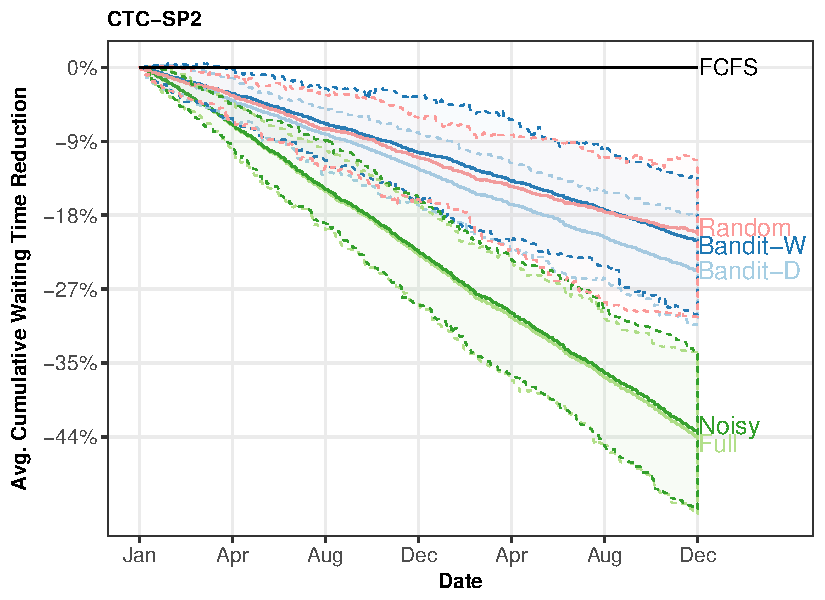
\includegraphics[scale=0.6]{figures/CTC-SP2.pdf}
  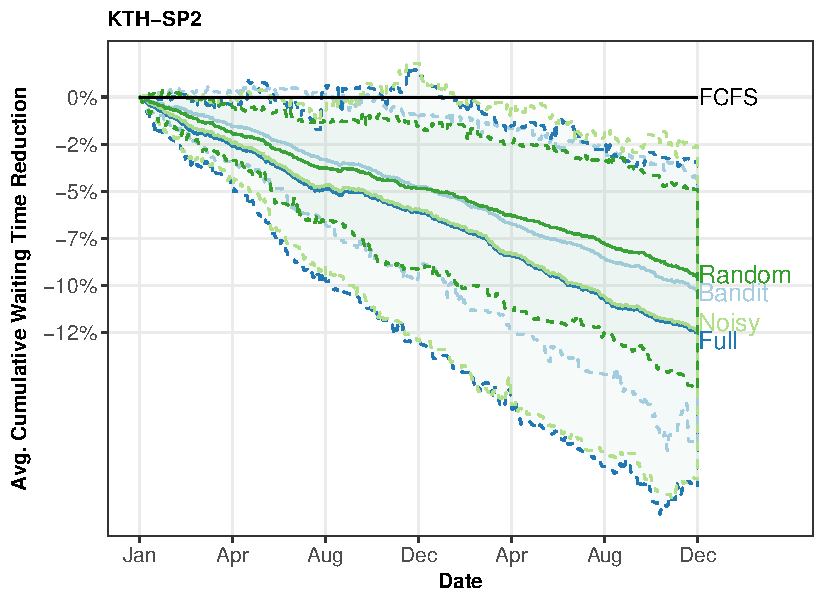
\includegraphics[scale=0.6]{figures/KTH-SP2.pdf}\\
  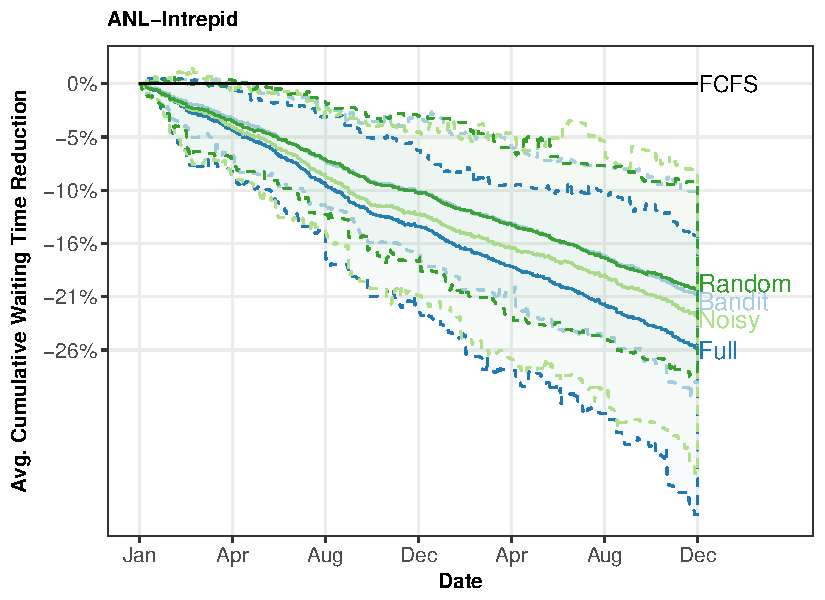
\includegraphics[scale=0.6]{figures/CEA-Curi.pdf}
  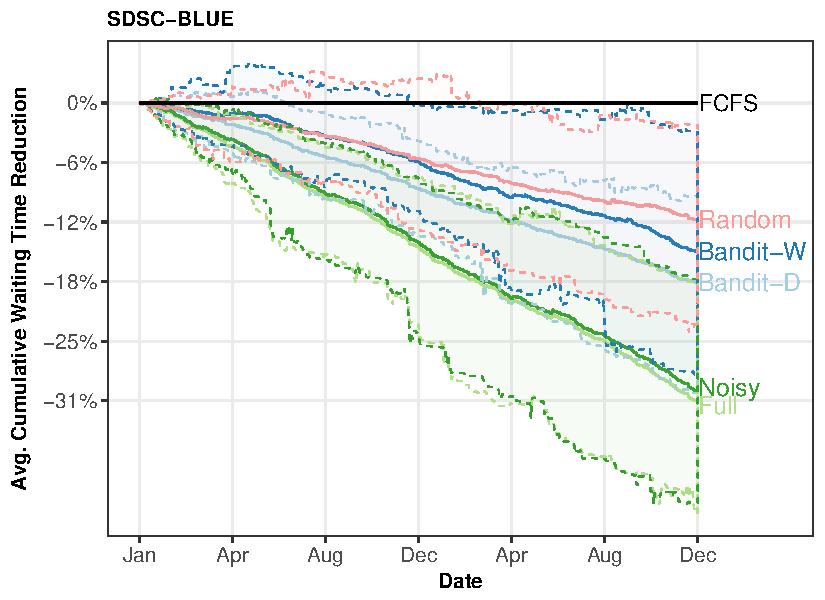
\includegraphics[scale=0.6]{figures/SDSC-BLU.pdf}\\
  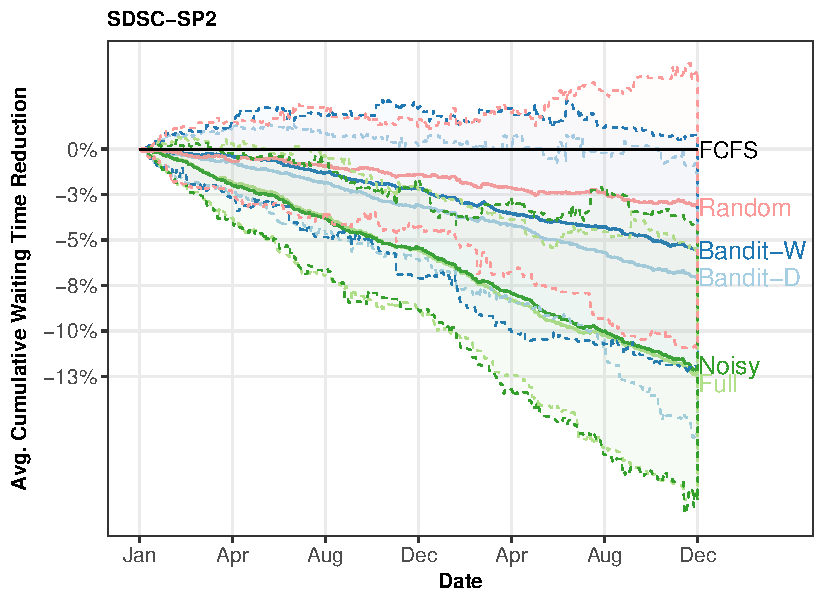
\includegraphics[scale=0.6]{figures/SDSC-SP2.pdf}
  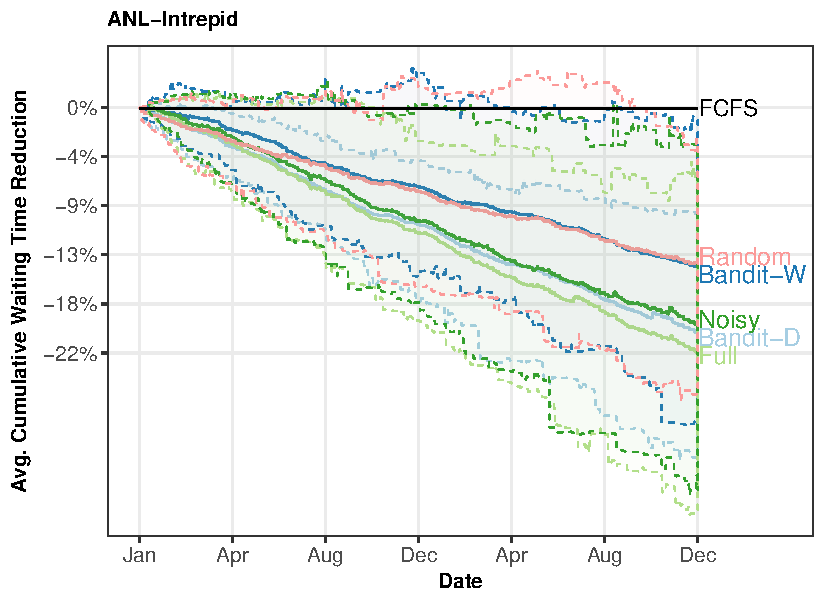
\includegraphics[scale=0.6]{figures/ANL-Intr.pdf}

  \caption{Evolution of the average cumulative waiting time improvement
    compared to EASY-FCFS of the FullFeedback, NoisyFeedback and EpsilonGreedy
    policies. The average is obtained by resampling the original trace 100
    times. The dashed lines represent the 10th and 90th percentiles of the
  values across this resampling. Each figure is a different trace, and this
figure is followed-up in figure~\ref{fig:follow} for the UniLu-Gaia log.}

  \label{fig:small}
\end{figure*}

\begin{figure}[]
  \centering
  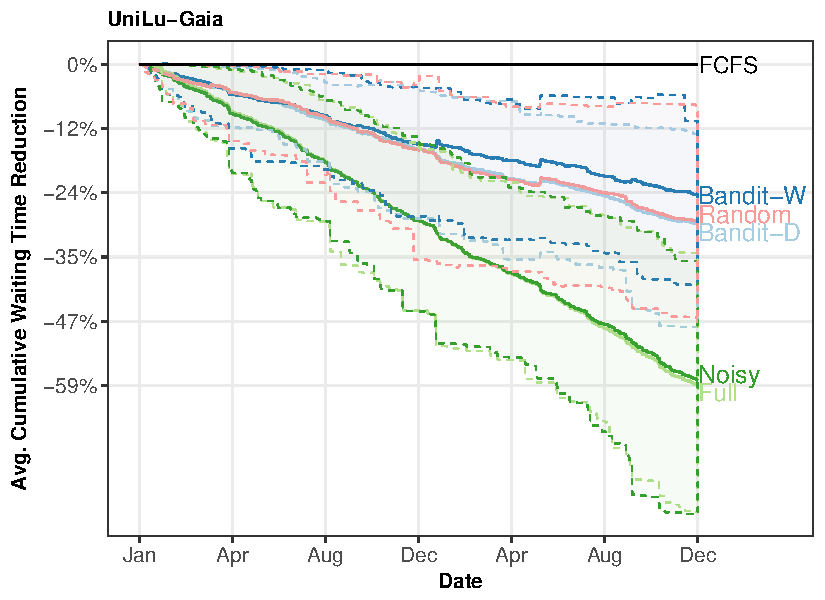
\includegraphics[scale=0.6]{figures/UniLu-Ga.pdf}

  \caption{Follow-up from figure~\ref{fig:small}, plot for the UniLu-Gaia log.}

  \label{fig:follow}
\end{figure}

Figures~\ref{fig:small} and~\ref{fig:follow} report the main experimental
result concerning the strategies proposed in this paper. These figures show the average cumulative improvement
of over EASY(FCFS,40h) of the three strategies we propose in the same format as Figure~\ref{fig:all}.
There are four strategies displayed on the graph:

\begin{itemize}
  \item Full (simulated) Feedback ($\Delta=$1 day)
  \item Noisy (simulated) Feedback ($\Delta=$1 day)
  \item Epsilon-Greedy (Bandit Feedback) ($\Delta=$1 day, $\epsilon=0.5$)
  \item Random $P \in P_i, 1 \le k \le 100$. ($\Delta=$1 day)
\end{itemize}

Observe that \textcolor{orange}{TODO lli  p sumlip sumlip llll sumli psumlips umlip sumil ip sumplip sumsl  ipsumul   ipsumm}.

\begin{table*}[]
  \centering
  \ra{1.3}
  \caption{Average Cumulative waiting time improvement with respect to EASY-FCFS of fixed policies.}
  \label{tab:strat}
  \begin{tabular}{@{}lrrrrrrrrrrr@{}}
    \hline
    Trace        & Random &      & Full &      & Noisy &      & Bandit &     \\
    \hline
    $\Delta$     & day    & week & day  & week & day   & week & day    & week\\
    CTC-SP2      & LCFS   & LPF  & SPF  & LQF  & SQF   & SEXP & LEXP   & LRF \\
    SDSC-SP2     & LCFS   & LPF  & SPF  & LQF  & SQF   & SEXP & LEXP   & LRF \\
    SDSC-BLUE    & LCFS   & LPF  & SPF  & LQF  & SQF   & SEXP & LEXP   & LRF \\
    ANL-Intrepid & LCFS   & LPF  & SPF  & LQF  & SQF   & SEXP & LEXP   & LRF \\
    CEA-Curie    & LCFS   & LPF  & SPF  & LQF  & SQF   & SEXP & LEXP   & LRF \\
    Unilu-Gaia   & LCFS   & LPF  & SPF  & LQF  & SQF   & SEXP & LEXP   & LRF \\
    \hline
  \end{tabular}
\end{table*}

Table~\ref{tab:strat} gives the performance of all variants for $\Delta=$ 1
day and $\Delta=$ 1 week.

Observe that \textcolor{orange}{TODO lli  p sumlip sumlip llll sumli psumlips umlip sumil ip sumplip sumsl  ipsumul   ipsumm}.

\begin{figure}[]
  \centering
  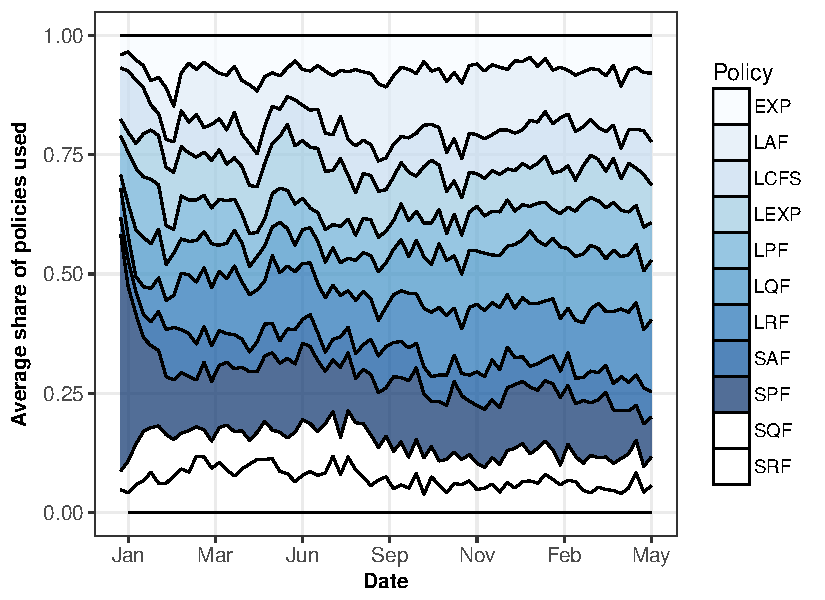
\includegraphics[scale=0.6]{figures/mosaicbandit-UniLu-Ga.pdf}

  \caption{Share of the policies chosen by Epsilon-Greedy as a function of
  time. The average choice is obtained by resampling the original trace 100
times and aggregating by date.}

  \label{fig:mosb}
\end{figure}

Figure~\ref{fig:mosb} gives insight regarding the behavior of the
Noisy (simulated) Feedback policy. This figure reports the share of the policies chosen
by the strategy on average as a function of time. This is an area plot, which means
that the height of the colored region represents the value. Moreover, the proportion of
times each policies are chosen by the strategy is aggregated across resampled traces.

Observe that \textcolor{orange}{TODO lli  p sumlip sumlip llll sumli psumlips umlip sumil ip sumplip sumsl  ipsumul   ipsumm}.

\begin{figure}[]
  \centering
  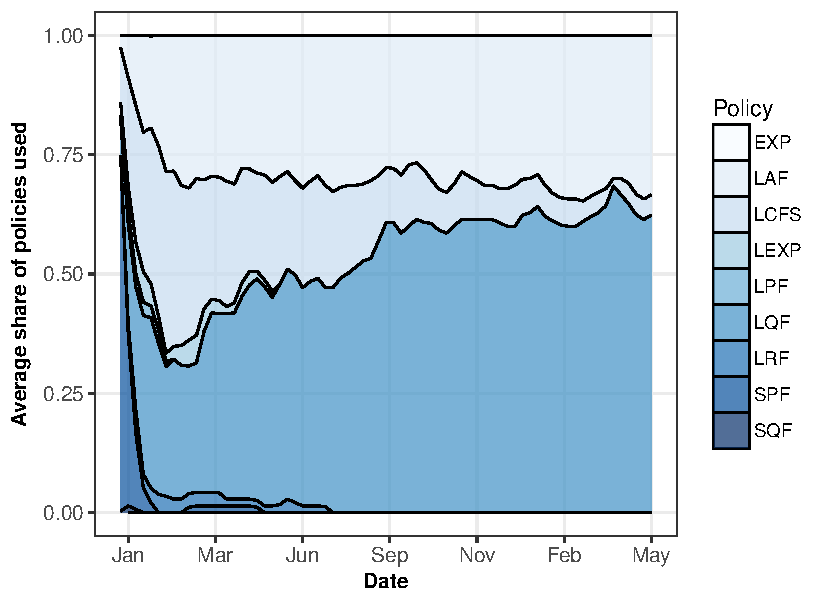
\includegraphics[scale=0.6]{figures/mosaic-UniLu-Ga.pdf}

  \caption{Share of the policies chosen by the Noisy policy. The average choice
  is obtained by resampling the original trace 100 times and aggregating by
  date.}

  \label{fig:mosn}
\end{figure}

Figure~\ref{fig:mosn} is the analogue of Figure~\ref{fig:mosb}, this time for
the Epsilon-Greedy policy.

Observe that \textcolor{orange}{TODO lli  p sumlip sumlip llll sumli psumlips umlip sumil ip sumplip sumsl  ipsumul   ipsumm}.

\section{Conclusion}
\label{sec:ccl}

The scheduling of parallel jobs on a given HPC platform is a very hard
optimization problem with many uncertain parameters. Even thought these
uncertainties could be reduced, determining efficient strategies remains
difficult.

We presented in this work a new way of addressing this problem.  The idea was
to look at the level of the scheduling process instead of trying to change its
parameters.

More precisely, we showed that it is worth to learn on the scheduling process
itself. Indeed, reordering the submission queues under EASY-BackFilling leads
to considerable gains in performance.

This approach was used in two methods: a method based on a simulator and a
method based on a multi-armed bandit algorithm. The first one provides very good results,
improving the average waiting times of the baseline FCFS ordering policy by a
factor of \textcolor{orange}{X} to \textcolor{orange}{X} The second one is
slighly less efficient with an improvement factor of  \textcolor{orange}{X} to
\textcolor{orange}{X}. However, it is more easy to use and less costly to run.

There are two directions for extensions of this work.  First, the question of
the existence of a more efficient selection strategy for bandit feedback for
these systems is not addressed by this work. Is a simulator really necessary?
%@Denis: a essayer.. 1 mois de travail pour tester?
Second, one can help but wonder what performance could be achieved by extending
the search space to arbitrary policies. This means doing a complete study
including lower bounding the cost and studying learning performance using some
function approximator.
%@Denis: c'est ce que font vasily et salah de deux manieres differentes.
%TODO SPLIT IN TWO, MENTION FACTOR ANALYSIS.
As these directions are data-bound, they will require careful application of
trace resampling techniques in order to be successful.

\begin{acks}

Authors are sorted in alphabetical order. The authors would like to warmly
thank Pierre Neyron for help with computational experiments and Arnaud Legrand
for discussions about reproducibility. We gracefully thank the contributors of
the Parallel Workloads Archive, Victor Hazlewood (SDSC SP2), Travis Earheart
and Nancy Wilkins-Diehr (SDSC Blue), Lars Malinowsky (KTH SP2), Dan Dwyer and
Steve Hotovy (CTC SP2), Joseph Emeras (CEA Curie and UniLu Gaia), Susan
Coghlan, Narayan Desay, Wei Tang (ANL Intrepid), and of course Dror Feitelson.
The Metacentrum workload log was graciously provided by the Czech National Grid
Infrastructure MetaCentrum. This work has been partially supported by the LabEx
PERSYVAL-Lab(\grantsponsor{ANR-11-LABX-0025-01}{ANR-11-LABX-0025-01}) funded by
the French program Investissement d'avenir.
\end{acks}

\bibliographystyle{acmst}
\bibliography{bibliography}

\clearpage

\section{artifact description: [online (bandit) policy selection for easy-backfilling]}

\subsection{Abstract}

This appendix describes the computational artifacts associated with this work. We
take a lightweight approach to replicability by packaging a declarative
workflow that generates all the figures from this paper and making it available
publicly. Moreover, questions regarding replication can be freely directed at
the authors via e-mail.

All the code associated with this work is released under the ~\cite{isc}
license as a persistent zenodo~\cite{zenodo} archive at~\cite{zenodomain}.

\subsection{Description}

There are various approaches for making computational experiments replicable,
among which distributing complete operating system images, containers, or
packaging software. As our experiments are cpu bound, we decide to opt for the
software packaging approach. This allows for replicating the experiments on clusters where virtualization is not
available or kernels are too old for containers old and decreases runtime.

All the dependencies of our
experiments (including our own code, dependencies for data processing and
visualization and workflow engine) are automatically managed by Nix up to the
actual execution of the code.

\subsubsection{Check-list (artifact meta information)}

{\small
\begin{itemize}
  \item {\bf algorithm: Scheduling Simulation Workflow}
  \item {\bf program: Ocaml, R, Bash, Zymake(all sources and dependencies included)}
  \item {\bf compilation: Ocaml 4.02.3, GNU bash version 4.4.5(1)-release, R version 3.3.2}
  \item {\bf transformations: Patched nix standard environment.}
  \item {\bf binary: Most binaries are cached by Nix channels.}
  \item {\bf data set: Traces from the parallel workload archive, included.}
  \item {\bf run-time environment: Nixpkgs 17.03}
  \item {\bf hardware: Dell PowerEdge R730}
  \item {\bf output: Files}
  \item {\bf experiment workflow: \lstinline[basicstyle=\ttfamily\color{blue}]|zymakefile|, see below}
  \item {\bf publicly available?: Open-Sourced under the ISC~\cite{isc} license.}
\end{itemize}
}

\subsubsection{Obtaining the code.}

\textbf{one-liner : replication}

Running the experiments can be done on any platform equipped with the nix
package manager by running:

\begin{lstlisting}
nix-build (fetchTarball ...)
\end{lstlisting}

\subsubsection{Hardware}

 Experiments presented in this paper were carried out using the Grid'5000
 testbed. Grid'5000 is supported by a scientific interest group hosted by Inria
 and including CNRS, RENATER and several Universities as well as other
 organizations\footnote{https://www.grid5000.fr}.  Access to the experimental
 machine(s) used in this paper was gracefully granted by research teams from
 LIG\footnote{http://www.liglab.fr} and Inria\footnote{http://www.inria.fr}.

 The experiments in this paper can run via in less than 24 hours on a
 moderately parallel host. More precisely, we had access to a Dell PowerEdge
 R730 equipped with a total of 56 threads @2.4GHz each and 757G of RAM. For
 this reason, the experimental campaign workflow was designed to be executed on
 a single host.

\subsubsection{Software dependencies}

All the software dependencies of our experiments are automatically managed by Nix.

\subsubsection{Datasets}

All data from this paper was obtained from the Swf Parallel Workloads
Archive~\cite{Feitelson20142967}. The data is cached in gzipped format in the
persistent archive associated with this workflow, should the Parallel
Workdloads Archive become unavailable.

\subsection{Installation}

The experiment dependencies are loaded into the environment by the
\lstinline[basicstyle=\ttfamily]|nix-build| command.

Nevertheless, the reader interested in using the tools outside the workflow can
obtain an environment by running the
\lstinline[basicstyle=\ttfamily]|nix-shell| command:

\begin{lstlisting}
nix-shell (fetchTarball ...)
\end{lstlisting}

Or alternatively, if the user is at the root of the extracted archive:

\begin{lstlisting}
nix-shell -A banditSelection
\end{lstlisting}

This allows to use the following command-line tools:

\begin{itemize}

  \item[ocs] The scheduling simulator used in the experiments. Use
    \lstinline[basicstyle=\ttfamily]|ocs --help| to see all available options.

  \item[ocs-sampler] The workload resampler used in the experiments. Use
    \lstinline[basicstyle=\ttfamily]|ocs-sampler --help| for usage.

  \item[zymake] The zymake~\cite{zymake} tool.
    The workflow can be executed in the current environment in parallel
    via \\ \lstinline[basicstyle=\ttfamily]|zymake -l localhost zymakefile|.

\end{itemize}

\subsection{Experiment workflow}

 All experiments are tied together using zymake~\cite{zymake}, a minimalistic
 workflow system designed for computational experiments\footnote{the zymake system
 is also packaged by our nix expressions.}. This system is
 analogous to a traditional build system with added workflow capabilities. The
 entire workflow that generates this article from the input data is contained
 in a single \lstinline[basicstyle=\ttfamily\color{blue}]|zymakefile| to be
 found at the root of the main archive. This workflow is composed of the
 following steps:

 \begin{itemize}
   \item[data]: Data extraction from archives, filtering, resampling.
     this is principally using shell scripts for data manipulation (see file
     \lstinline[basicstyle=\ttfamily\color{blue}]|misc/strong\_filter| for the
     filtering steps used) and ocaml code that implements the resampling method
     described in~\ref{ssub:resampling}.

   \item[simulation]: This step runs the lightweight ocaml backfilling
     simulator specially written for this work. this simulator is made
     available under the isc~\cite{isc} license both as a persistent zenodo
     archive at~\cite{ocst} and as a git repository at ~\cite{ocstgit}.

   \item[analysis]: This step runs r code that generates the figures
     presented in this paper.
 \end{itemize}


\subsection{Evaluation and expected result}

All resulting figures will be situated in the simlinked folder named
\lstinline[basicstyle=\ttfamily\color{blue}]|result| positionned at the root of
the archive.

\subsection{Experiment customization}

Readers interested with modifying the experiments can obtain the zenodo archive
at \url{https://truc.tgz}

The experiments are replicated with the same procedure as before, this time
invoking the build command with the local folder:

\begin{lstlisting}
nix-build -A banditSelection
\end{lstlisting}

The file tree has the following structure:

\dirtree{%
  .1 root .
.2 zymakefile \textcolor{brown}{Zymake workflow} .
.2 default.nix \textcolor{brown}{Nix packaging} .
.2 pkgs/ \textcolor{brown}{Nix packaging} .
.2 gz/ \textcolor{brown}{Data archive} .
.3 ANL-Intrepid.swf.gz .
.3 $\cdots$ .
.2 misc/ \textcolor{brown}{Visualization and filtering code} .
.2 ocst/ \textcolor{brown}{Simulator Code} .
.2 paper/ \textcolor{brown}{This article.} .
}

Most simple workflow modifications (using different traces, changing the sample
sizes) can be obtained by modifying the
\lstinline[basicstyle=\ttfamily\color{blue}]|zymakefile|. For modification

\subsection{Notes}

This artefact description was prepared according to the guidelines located at
\url{http://ctuning.org/ae/submission.html}

\end{document}
